% Copyright (c) 2014,2016 Casper Ti. Vector

\chapter{系統測試}

本論文將開發讓商家能夠結合商品與RFID標籤,以達到快速建構與管理商品資料庫之系統,並且讓商家及顧客可以運用手機NFC功能來實際運作比特幣的行動支付流程。店家只需要掃描商品上的RFID標籤,即可快速建立交易清單,再利用NFC功能與顧客之行動裝置進行訊息交換,輕鬆地將商家的收款地址以及交易資料傳送給顧客,收到資料後便能快速地以顧客之比特幣行動電子錢包付款,並將交易細項儲存下來,以便未來商家與顧客能夠快速查詢比特幣行動支付的交易紀錄。
本系統主要是以完成區塊鏈之數位加密貨幣的收款監督系統為主要目標,本論文進而將積極利用自由軟體的利基:使用成本低、進入門檻低、開放原始碼、社群能力強、共通性及移植性強、資通安全性高等優勢來開發本論文收款監督系統的應用服務平台。
本專案範圍包含建置下面主系統與各項子系統,主系統為:
		\paragraph{基於區塊鏈技術的收款監督系統(Blockchain-based Payment Collection Supervision system, BPCS)}

各子系統分別為:
 		\paragraph{商家端建置與管理商品資訊子系統(Store and Merchandise Information Management Sub-System,SMIMSS)}本系統可以讓商家在進貨時,快速地將RFID標籤之識別碼與進貨商品資訊整合在一起,並且透過本系統新增、修改或刪除資料庫內部的資訊,包括產品名稱、詳細資訊,存貨數量等資訊,商家與顧客便可依照該資料庫取得當前商品資訊與狀態。不僅讓商店的存貨資訊更加清楚明瞭,也可以提供顧客更多的即時服務。
 		\paragraph{商家端行動收銀與交易明細系統(Store Mobile payment Collection and Transaction Sub-System,SMCTSS)}本系統使商家在結帳時,能夠以手機NFC功能掃描商品上的RFID 標籤,即可簡單地建立交易清單,並透過NFC與顧客手機碰觸,將交易清單以及商家之比特幣收款地址等等重要交易資訊一併傳遞給顧客,可以簡短結帳的速度,使結帳效率大幅提升。 
 		\paragraph{顧客端行動支付與交易明細系統(Client Mobile Payment and Transaction Sub-System,CMPTSS)}顧客在結帳時,不必再麻煩的拿出信用卡或是零錢包,只需要拿出手機讓店員以NFC將交易清單與比特幣地址轉送給自己,即可自動連結至比特幣電子錢包的應用程式當中,並且自動填妥相關資料,如:交易金額、收款地址等等與此同時也能將交易紀錄儲存於客戶端,以便日後顧客快速取得過往的交易紀錄,除此之外亦可讓廣大的民眾體驗數位加密貨幣與行動支付帶來的便利生活。

 	\section{測試說明}

 	\subsection{測試範圍}
 	本文件主要是描述基於區塊鏈技術的收款監督系統的測試計畫。確認在系統整合前,必須先確認所有的設計元件均可正確的輸出,在此我們著重於整合系統測試 (Integration Test) 及接受度測試 (Acceptance Test)。本文件內容將依據系統需求規格書與系統設計文件,描述關於整合測試的相關計畫與內容。並希望透過此文件之描述與實踐,達到順利進行測試工作之目的。

 	\subsection{驗收標準}
 	本測試計劃需要滿足下列的測試接受準則: 

 	\begin{enumerate}
		\item 本系統需要對所有列為必要(Critical、Important、Desirable)之需求作完整測試。
		\item 測試程序需要依照本測試計畫所訂定的程序進行,所有測試結果需要能符合預期測試結果方能接受。
		\item 以測試案例為單位,當測試未通過時,需要進行該單元的測試,其接受的準則與前一項規定相同。 
	\end{enumerate}
 	
 	\section{測試環境}

 		\subsection{硬件規格}
 			\paragraph{系統主機}一台以上主機,每台主機CPU為Intel P4 1.0GHz或以上,256 MB RAM或以上,60G以上硬碟空間。
 			\paragraph{周邊設備}一台以上智慧型手機,與用來代表虛擬商品的數個RFID標籤;已可供測試NFC用的智慧型手機包含小米3 WCDMA版與Google Nexus 5。

 		\subsection{軟件規格}
 		關於測試環境所需的軟體規格說明,如下列所示:作業系統:Window 10、Android 6.0.1/7.1.1

 		\subsection{測試數據源}
 		在銘傳大學桃園校區資工系實驗室,由本計畫主持人及助理人員透過Android手機進行的交易模擬實驗,測試環境如圖\ref{fig4}的示意。

 	\section{測試計劃和程序}

 		\subsection{測試時間規劃}

 		\paragraph{時程}

 			\begin{enumerate}
 				\item 各子系統之內部元件整合測試 (Module Test)(106/2/25~106/6/8)
 				\item 基於區塊鏈技術的收款監督系統整合測試 (Integration Test) (106/6/8~106/6/21)
 				\item 基於區塊鏈技術的收款監督系統接受度測試 (Acceptance Test) (106/7/10~106/7/21)
			\end{enumerate}

		\paragraph{查核點}

			\begin{enumerate}
 				\item 各子系統之內部元件整合測試 (Module Test)(106/5/10)
 				\item 基於區塊鏈技術的收款監督系統整合測試 (Integration Test) (106/7/1)
 				\item 基於區塊鏈技術的收款監督系統接受度測試 (Acceptance Test) (106/7/1)
 			\end{enumerate}

 		\subsection{集成測試(Integration Testing)}
 			\begin{figure}[h]
				\centering
				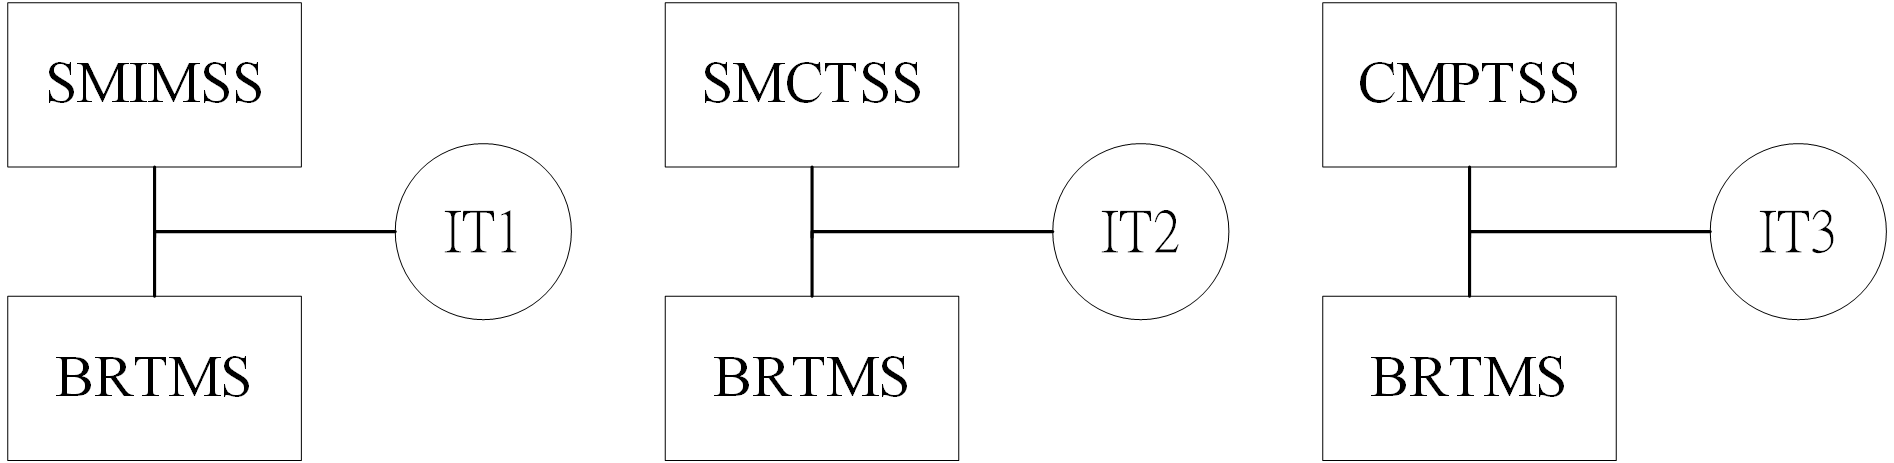
\includegraphics[width = 1\textwidth]{IntegrationTesting.png}
				\caption{整合子系統測試}\label{IntegrationTesting}
			\end{figure}

		\subsection{驗收測試(Acceptance Testing)}
		本系統須達成使用案例(use case)所列功能:
			\begin{figure}[h]
				\centering
				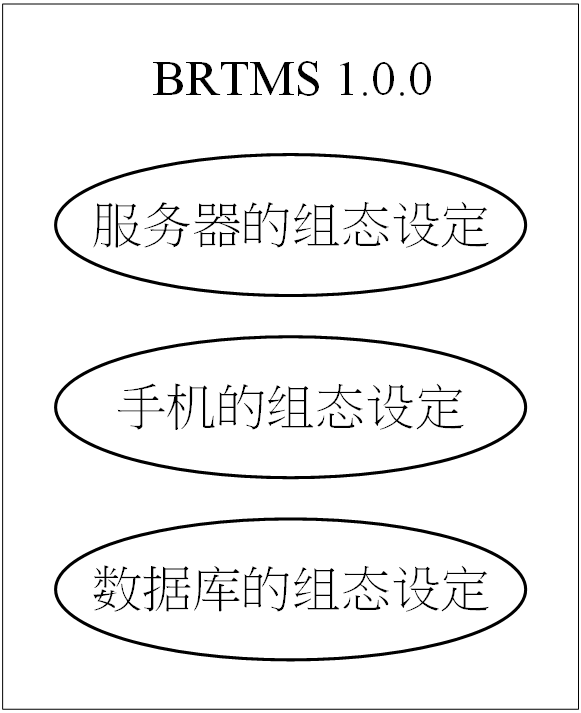
\includegraphics[width = 0.6\textwidth]{usecasediagram.png}
				\caption{BRTMS使用案例圖}\label{usecasediagram}
			\end{figure}



	\section{區塊鏈的實名交易監督系統實驗}
	根據比特幣點對點架構,儘管客戶和商店之間的交易細節已經快速存儲到雲數據庫,但官方確認交易與當前比特幣區塊鏈的交易通常需要更長的時間,因為需要確保確認的數量在交易廣播比特幣點對點網絡並存儲到緩存池後,是否存在雙重支付。
	因此,為了驗證我們提出的BRTMS不會通過使用比特幣等加密貨幣影響交易完成時間,我們於2017年7月25日在Testnet實驗中連續記錄了30筆交易信息。首先,我們使用區塊鏈檢視器(Blockchain Explorer)\supercite{Blockchainexplorer:Ananalyticalprocessandinvestigationenvironmentforbitcoin},如\ref{fig9}的第一張快照所示,透過使用Testnet依序進行30筆比特幣交易,如圖\ref{fig9}的中間快照所示,最後30筆交易完成時間全部記錄在區塊鏈檢視器。實驗結果顯示,實驗中的所有交易都在3秒鐘左右(平均2.97秒,標準差小於1秒)發送到比特幣網絡緩存池,平均交易完成時間在比特幣區塊鏈中確認為522.33秒(小於9分鐘),標準差大約為339秒。根據比特幣Testnet上的初步實驗結果顯示,我們提出的BRTMS可以快速有效地執行區塊鏈支付收款監督。

	\begin{figure}[h]
		\centering
		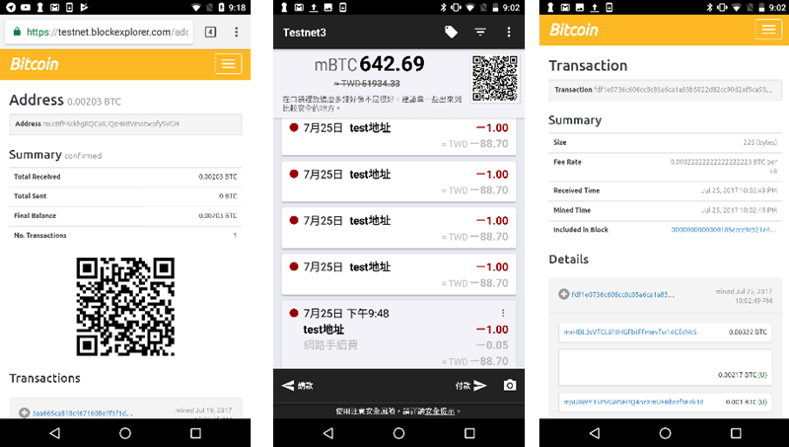
\includegraphics[width = 0.7\textwidth]{fig9.png}
		\caption{使用區塊鏈瀏覽器驗證存儲在比特幣區塊鏈中的交易過程}\label{fig9}
	\end{figure}

	\section{多重簽章優化區塊鏈的實名交易監督系統實驗}
		\subsection{交易效能實驗}
		本節主要介紹比特幣測試幣於Green Address錢包進行交易的效能實驗與結果分析,包含該實驗的目的、方法及結果分析。

			\paragraph{實驗目的}實驗的目的是要確認我們的系統在商家端進行行動支付時能快速、精準且高效率的進行交易,並瞭解使用一般Testnet錢包與Green Address錢包作為交易媒介的確認交易時間的差距。
			\paragraph{實驗方法}本次的實驗分為兩部份,分別是透過比特幣 Testnet錢包以及使用本論文所採用的Green Address 比特幣 錢包上執行25次付款,皆以相同地址收款,交易金額都設定為0.00001BTC, 實驗時間為2017年9月6日-17:00~17:50,每隔兩分鐘執行一次付款的動作,總共歷時50分鐘。兩款錢包同時發起交易,並透過區塊鏈檢視器進行記錄時間,最後再比較使用一般比特幣錢包及Green Address錢包兩者之間的差距。
			\paragraph{實驗結果}本次實驗分別記錄以Testnet錢包及Green Address錢包執行25次交易的進入緩存池等待時間和寫入區塊等待時間。若以Testnet錢包交易,必須等到交易寫入才能保證此筆交易不會被礦工遺棄,也才算真的完成這筆交易;但若以Green Address錢包發起交易就大不相同,當交易進入緩存池,即使遇到交易被礦工遺棄的情況,Green Address機構節點也會重新發起此筆交易,保證讓交易寫入區塊,所以只要進入緩存池我們就可以視為交易完成,透過兩者錢包的交易數據,我們比較及分析兩種錢包交易的時間數據。

%			\begin{figure}[h]
%				\centering
%				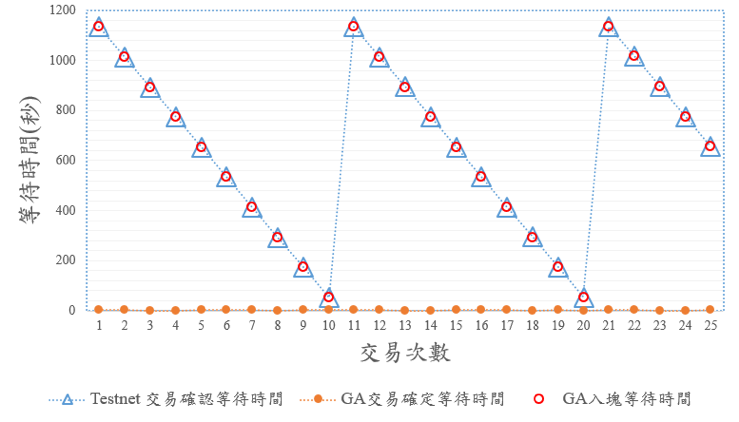
\includegraphics[width = 0.7\textwidth]{fig12.png}
%				\caption{fig12}\label{fig12}
%			\end{figure}

透過本次的實驗,我們可以發現雖然以兩種錢包交易進入區塊的等待時間完全相同,但因為Green Address錢包的特性,只要進入緩存池就算完成交易確認,因此Green Address錢包的完成交易確認的時間遠遠快於一般Testnet。相信以此⽅式作為主要⽀付管道,可以省去消費者在現金⽀付時掏零錢、算錢及找零等繁瑣的動作及時間,以此達成提升⽇常⽣活中的便利性與安全性。